
\section{训练成本对比}
Semi-OPD 更快，因为轨迹生成和教师评分在训练前仅需执行一次。与 Lightning OPD~\citep{wu2026lightning} 类似，这消除了训练环中的在线轨迹生成和教师推理，因此所有 GPU 都可用于轨迹生成、教师对数概率评分以及学生训练。对于固定的学⽣，相同的轨迹缓存也可在不同教师之间重复使用；评估新教师只需计算其在已缓存轨迹上的对数概率。这在实践中可进一步降低比较或选择教师的成本。相比之下，Relay-OPD 在整个训练过程中需要交替进行学生和教师的生成，导致更高的训练成本。

\begin{table*}[h]
  \centering
  \caption{\textbf{训练成本。} 100个训练步骤的H100 GPU小时数，不包括评估。
  Semi-OPD的成本是滚动生成、教师评分和学生训练之和。
  FastOPD是将滚动截断至4K token的OPD。加速比为该方法的GPU小时数除以Semi-OPD的GPU小时数。}
  \vspace{2mm}
  \label{tab:speedup}
  \setlength{\tabcolsep}{10pt}
  \renewcommand{\arraystretch}{1.15}
  \begin{tabular}{@{}lrr@{}}
    \toprule
    Method & GPU-hours & Semi-OPD speedup \\
    \midrule
    \multicolumn{3}{@{}l}{\textit{Qwen3-1.7B (non-thinking) $\leftarrow$ Qwen3-4B-Instruct-2507}$^{\dagger}$} \\
    \quad Relay-OPD & 173.3 & $34.7\times$ \\
    \quad OPD       & 56.8  & $11.4\times$ \\
    \quad FastOPD   & 11.7  & $2.3\times$ \\
    \quad \textbf{Semi-OPD} & \textbf{5.0} & -- \\
    \midrule
    \multicolumn{3}{@{}l}{\textit{Qwen3-4B (non-thinking) $\leftarrow$ Qwen3-30B-A3B-Instruct-2507}$^{\dagger}$} \\
    \quad Relay-OPD & 604.4 & $19.5\times$ \\
    \quad OPD       & 199.1 & $6.4\times$ \\
    \quad FastOPD   & 77.3  & $2.5\times$ \\
    \quad \textbf{Semi-OPD} & \textbf{31.0} & -- \\
    \midrule
    \multicolumn{3}{@{}l}{\textit{Qwen3-14B (thinking) $\leftarrow$ Qwen3-235B-A22B-Thinking-2507}} \\
    \quad Relay-OPD & 1546.5 & $24.6\times$ \\
    \quad OPD       & 480.0  & $7.6\times$ \\
    \quad FastOPD   & 169.8  & $2.7\times$ \\
    \quad \textbf{Semi-OPD} & \textbf{63.0} & -- \\
    \midrule
    \multicolumn{3}{@{}l}{\textit{Nemotron-Cascade-2-30B-A3B $\leftarrow$ Nemotron-Cascade-2-Math-Expert}} \\
    \quad Relay-OPD & 933.5 & $14.1\times$ \\
    \quad OPD       & 301.4 & $4.5\times$ \\
    \quad FastOPD   & 147.5 & $2.2\times$ \\
    \quad \textbf{Semi-OPD} & \textbf{66.4} & -- \\
    \bottomrule
  \end{tabular}\\[4pt]
  \begin{minipage}{0.85\linewidth}
  \footnotesize
  $^{\dagger}$ Semi-OPD 在这些数据对上使用 4K 训练滚动数据，而 OPD 使用 16K；在另外两组数据对上，两者均使用 16K。训练滚动数据上限列于 \cref{tab:allpairs}。\\
  \end{minipage}
\end{table*}


\clearpage
\newpage
\section{长度与自我修正膨胀}
\label{app:inflation}

图~\ref{fig:inflation} 跟踪了每种方法在训练过程中生成的轨迹的两个属性：轨迹长度（每个轨迹的平均生成 token 数）和自我修正词密度。在 OPD 情况下，当前学生会在每一步重新生成轨迹；在 Semi-OPD 情况下，这些轨迹是来自初始学生的冻结样本 $\pi_0$。

\paragraph{测量自我纠正能力。}
我们使用词汇密度来衡量自我修正。我们在生成的补全内容（不包括提示）中，统计一组固定自我修正词汇的不区分大小写、完整单词出现次数，即 \{\textit{wait, but, hmm, actually, hold, however, yet, oh, alternatively, no, ah, oops, well}\}。在每个训练步骤中，我们汇总全部 128 个训练回溯路径，并报告 $1000 \times \sum_i h_i / \sum_i c_i$ ，其中 $h_i$ 表示词频命中数，$c_i$ 表示回溯路径中的字符数，$i$ 为回溯路径编号。教师参考结果（虚线）在同一训练步骤最终提示上，对 128 个教师样本（$T{=}1.0$ ，相同的回溯路径上限）采用相同定义；教师的回溯长度也在相同样本上进行测量。由于词表包含 \textit{but} 和 \textit{no} 等常见话语词，该指标是反思性、犹豫式表达风格的代理度量，而非已验证修正次数的直接计数。我们在附录~\ref{app:qualitative} 中展示了 OPD 与 Semi-OPD 回溯路径对比的更多定性示例。

\begin{figure*}[h]
    \centering
    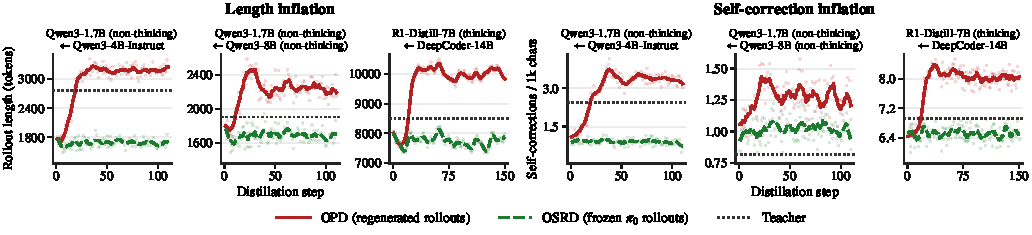
\includegraphics[width=\linewidth]{figures/fig_inflation.pdf}
    \caption{\textbf{同策略回溯在OPD期间被放大。}
    训练回溯的回溯长度（左侧三个面板）和自我修正词密度（右侧三个面板）。OPD回溯变得更长并使用更多的自我修正词，最终超过教师（虚线），而从初始学生 $\pi_0$ 一次性采样的冻结回溯则没有。}
    \label{fig:inflation}
\end{figure*}

\clearpage
\newpage
\section{定性示例：OPD 与半 OPD 训练部署}
\label{app:qualitative}



\providecommand{\refl}[1]{\textcolor{red}{\textbf{#1}}}
\providecommand{\capped}{{\color{gray}\textit{[generation cap reached; no final answer]}}}
\providecommand{\gap}[1]{{\color{gray}\textit{[\,\dots\ #1 tokens omitted\,\dots]}}}
\newtcolorbox{qualproblem}{colback=gray!6,colframe=gray!50,boxrule=0.4pt,arc=1pt,
  left=3pt,right=3pt,top=2pt,bottom=2pt,fontupper=\footnotesize}
\newtcolorbox{Semi-OPDbox}[1]{colback=white,colframe=green!45!black,boxrule=0.5pt,arc=1pt,
  left=2pt,right=2pt,top=1pt,bottom=1pt,toptitle=1pt,bottomtitle=1pt,
  fonttitle=\scriptsize\bfseries,fontupper=\scriptsize,title={#1},
  before upper={\setlength{\parskip}{2pt}\setlength{\parindent}{0pt}}}
\newtcolorbox{opdbox}[1]{colback=white,colframe=black!65,boxrule=0.5pt,arc=1pt,
  left=2pt,right=2pt,top=1pt,bottom=1pt,toptitle=1pt,bottomtitle=1pt,
  fonttitle=\scriptsize\bfseries,fontupper=\scriptsize,title={#1},
  before upper={\setlength{\parskip}{2pt}\setlength{\parindent}{0pt}}}



\begin{figure*}[h]
\centering
\begin{qualproblem}
\textbf{Example 1.} Qwen3-1.7B $\leftarrow$ Qwen3-30B-A3B-Thinking (thinking). OPD rollout at training step 201; Semi-OPD rollout from $\pi_0$; generation cap 16{,}384 tokens.\par\smallskip
\textbf{Problem.} What is the hundreds digit of the sum below?

$1 + 12 + 123 + 1234 + 12345 + 123456 + 1234567 + 12345678 + 123456789$
\end{qualproblem}
\vspace{-1pt}
\begin{minipage}[t]{0.495\linewidth}\vspace{0pt}
\begin{Semi-OPDbox}{Semi-OPD (frozen $\pi_0$ rollout): 5{,}688 tokens, 36 reflection words, reaches an answer}
\gap{1{,}101}

现在，对1000取模：205。

\refl{Wait}, so the total sum mod 1000 is 205? So the last three digits of the sum are 205. Therefore, the hundreds digit is 2. Is that correct?

\gap{2{,}535}

总计为137,174,205。

现在，最后三位数字是205，因此百位数字是2。这样就确认了。

\gap{1{,}380}

因此，和的百位数字是2。

\textbf{最终答案} \newline\rule{0pt}{2.6ex}$\boxed{2}$

\gap{550}
\end{Semi-OPDbox}
\end{minipage}\hfill
\begin{minipage}[t]{0.495\linewidth}\vspace{0pt}
\begin{opdbox}{OPD（步骤201）：16,384个token，80个反射词，达到上限}
\gap{6,594}

百位数字之和：0+0+1+2+3+4+5+6+7 = 28

加上十位的进位：28 + 4 = 32

和的百位数字：32 mod 10 = 2

\gap{2,658}

现在，和的百位是右边第二个数字，因此32 mod 100为32，所以百位数字是3

\gap{2,458}

\refl{啊}！这里有个错误：当我提到百位数字之和是28，加上十位的进位（4），这是百位的总和，即32。 \refl{但} 和的百位数字是32的个位数字，也就是2，而进位是3（进到千位）。

\gap{3,097}

\refl{等等}，不对。32是百位数字之和（加上进位）的结果，这表示百位的总值。例如，如果百位的和是32，意味着总和在百位上有3，在十位上有2？ \refl{不对}，数位的含义是：

- 如果百位的和是32，这意味着你有3×100 + 2×1，所以百位数字是3，十位数字是2。

\gap{1,140}

举个例子，如果百位数字之和加上进位是32，那么总值是32×100 +（余数），所以百位数字是2（即32的十位）。

\refl{等等}，不对：如果百位数字之和加上进位是32，那么百位对总和的贡献值是32×100。 \refl{但} 实际上，在加法中，百位是百位数，所以百位数字是总和中百位上的数字。

\capped
\end{opdbox}
\end{minipage}

\label{fig:qual_t1}
\end{figure*}







\begin{figure*}[p]
\centering
\begin{qualproblem}
\textbf{Example 2.} DeepSeek-R1-Distill-Qwen-7B $\leftarrow$ DeepCoder-14B (thinking). OPD rollout at training step 128; Semi-OPD rollout from $\pi_0$; generation cap 16{,}384 tokens.\par\smallskip
\textbf{Problem.} Find the positive solution to \newline $\frac 1{x^2-10x-29}+\frac1{x^2-10x-45}-\frac 2{x^2-10x-69}=0.$
\end{qualproblem}
\vspace{-1pt}
\begin{minipage}[t]{0.495\linewidth}\vspace{0pt}
\begin{Semi-OPDbox}{半开放问题解决框（冻结 $\pi_0$ 推演）：2{,}228 个 token，10 个反思词，得出答案}
\gap{176}

让我设 $y = x^2 - 10x$ 。于是，每个分母变为 $y - 29$ ，$y - 45$ ，和 $y - 69$ 。因此代入后，方程变为：

$\frac{1}{y - 29} + \frac{1}{y - 45} - \frac{2}{y - 69} = 0.$ 

\gap{769}

因此，方程简化为：

-64y +2496=0。

\gap{718}

\refl{但}题目要求正解，所以 x=13。

\gap{438}
\end{Semi-OPDbox}
\end{minipage}\hfill
\begin{minipage}[t]{0.495\linewidth}\vspace{0pt}
\begin{opdbox}{OPD（步骤128）：9{,}016个token，117个反射词，得出答案}
\gap{124}

我们设 $y = x^2 - 10x$ 。这似乎是一个聪明的置换，因为每个分母都可以用 y 表示。

\gap{1{,}916}

\refl{等等}，也许这是一个完全平方？让我检查一下257,664是否是平方数。

\refl{嗯}，508$^2$ =258,064。

507$^2$ =257,049。

相减得 257,664 -257,049=615。

不是完全平方。\refl{嗯}\dots{} \refl{等等}，也许615可以表示为……还不确定。

\gap{735}

\refl{等等}，也许最初的方法让我卡住了，因为平方根太复杂了。可能我之前计算有误？让我回头检查一下。

\refl{等等}，\refl{稍等}。让我重新梳理一下：

\gap{139}

\refl{等等}，\refl{稍等}，也许我在展开分母时出错了？

\refl{等等}，(y -29)(y -45)= y$^2$  -45y -29y +29$\times$ 45= y$^2$  -74y +1305？

\refl{等等}，29$\times$ 45：20$\times$ 45=900，9$\times$ 45=405，合计1305，这是正确的。

\refl{等等}，我之前交叉相乘时会不会犯了错误？让我再仔细核对一遍。

\gap{5{,}172}

因此，好的，逻辑成立。

步骤：代入 y=x$^2$  -10x，将方程化为仅含 y 的形式，解得 y=39，求得 x=13 和 x=-3，识别出所需解为正数。

因此，正解是13。

\gap{587}
\end{opdbox}
\end{minipage}

\label{fig:qual_ds7}
\end{figure*}


\begin{figure*}[p]
\centering
\begin{qualproblem}
\textbf{Example 3.} Qwen3-1.7B $\leftarrow$ Qwen3-30B-A3B-Instruct-2507 (non-thinking). OPD rollout at training step 90; Semi-OPD rollout from $\pi_0$; generation cap 4{,}096 tokens.\par\smallskip
\textbf{Problem.} Let $f(x) = \frac{x+1}{x-1}$. Then for $x^2 \neq 1$, find the expression for $f(-x)$. The original answer is in $\frac{k}{m}$ format, please give the value of $k + m$.
\end{qualproblem}
\vspace{-1pt}
\begin{minipage}[t]{0.495\linewidth}\vspace{0pt}
\begin{Semi-OPDbox}{半开放问题求解（冻结 $\pi_0$ 展开）：308 token，0 个反思词，得出答案}
\gap{69}

第 1 步：将 $-x$ 代入 $f(x)$

$f(-x) = \frac{(-x) + 1}{(-x) - 1}$

化简分子和分母：

$f(-x) = \frac{-x + 1}{-x - 1}$

我们可以从分子和分母中同时提出一个负号：

$f(-x) = \frac{-(x - 1)}{-(x + 1)} = \frac{x - 1}{x + 1}$

第 2 步：识别 $k$ 和 $m$

我们有：

$f(-x) = \frac{x - 1}{x + 1}$

这已经符合 $\frac{k}{m}$ 的形式，其中：

$k = -1,\allowbreak \quad m = 1$

第 3 步：计算 $k + m$

$k + m = -1 + 1 = \boxed{0}$

最终答案：

$\boxed{0}$
\end{Semi-OPDbox}
\end{minipage}\hfill
\begin{minipage}[t]{0.495\linewidth}\vspace{0pt}
\begin{opdbox}{OPD（步骤90）：4{,}096个token，87个反射词，达到上限}
\gap{239}

步骤3：检查其是否符合$\frac{k}{m}$的形式

这并非一个常数，而是一个关于$x$的有理函数，但我们需假设其形式为$\frac{k}{m}$，即一个常数。\refl{等等}——也许我们理解错了？

\gap{156}

\refl{等等}——但$f(-x)$并不是一个常数函数。只有当$x$是常数时才成立——但$x$是一个变量。

除非——也许题目是个陷阱？

\refl{等等}——让我们重新核对一下。

\gap{151}

\refl{等等}——也许题目并非要求$f(-x)$，而是要求将$f(-x)$的表达式化简为一个常数形式？

\refl{等等}——但$f(-x) = \frac{x - 1}{x + 1}$并不恒为常数。

\gap{510}

\refl{等等}——\textbf{也许原题存在笔误？}

\gap{531}

\refl{等等}——继续推进。

\refl{等等}——\textbf{假设原始答案是$\frac{1}{2}$}

\gap{466}

\refl{等等}——\textbf{终于！} 假设题目表述有误。

\gap{1{,}658}

\refl{等等}——也许原本应该是求$f(-x)$在特定$x$处的\textbf{值}？\refl{但}不是。

\refl{等等}——也许题目是在要求用$f(x)$表示$f(-x)$的表达式？

\gap{100}

\capped
\end{opdbox}
\end{minipage}

\label{fig:qual_q30i}
\end{figure*}

\FloatBarrier
